\documentclass{scrartcl}
\usepackage[utf8]{inputenc}
\usepackage[english]{babel} % Trennung nach der neuen deutschen Rechtschreibung
\usepackage[utf8]{inputenc}
\usepackage[T1]{fontenc}
\usepackage{lmodern}
\usepackage{subcaption}
\usepackage{chemformula}
\usepackage{placeins}
\usepackage{multirow}
\usepackage{enumitem}
\usepackage{amssymb}
\usepackage{amsmath} % Erweiterte Mathematik-Umgebung
\usepackage{amsfonts} % zusätzliche Mathematik-Schrifttypen (v.a. \mathbb für Mengen)
\usepackage{ulem}
\usepackage{amsthm}
\usepackage{graphics}%soll beim Graphiken einfügen hilfreich sein
\usepackage{graphicx}
\usepackage{wrapfig}%lässt Textumflossene Bildeinbindung zu
\usepackage{epstopdf}%soll eps in pdf umwandeln
\usepackage{placeins}
\usepackage{amsthm}
\usepackage{subcaption}
\usepackage{wrapfig}
\usepackage{float}
\usepackage{hyperref}
\usepackage{ragged2e}

\usepackage{floatrow}
% Table float box with bottom caption, box width adjusted to content
%\newfloatcommand{capbtabbox}{table}[][\FBwidth]

\usepackage[a4paper, portrait, margin=2.5cm]{geometry}

\setlength\parindent{0pt}

\begin{document}

\begin{titlepage}
    \begin{center}
        \vspace*{1cm}
        \Huge
        \textbf{Thermal Conductivity of Aluminium}
        
        \vspace{0.5cm}
        \LARGE
        
        
        \vspace{0.5cm}
        \LARGE
        Advanced Lab Course
        
        \vspace{1.5cm}
        \textbf{Louis-Hendrik Barboutie (020157041C), Frederik Ehl (0201719742) and Florence Schmerber (0201845640)}
        
        \vspace{1cm}
        Supervisor: Himanshu PHIRKE
        \vfill
        

        
\includegraphics[width=0.4\textwidth]{logo_uni.jpg}
        
        \Large
        $12^{\underline{\text{th}}}$ May 2022
    \end{center}
\end{titlepage}



\section{Introduction}
In today experiment, we are interested in studying the thermal conductivity of aluminium, in other words the ability to conduct heat. Metals have a high thermal conductivity, since they have free electrons that can freely move throughout the material and therefore transfer thermal energy, compared to isolators that have low thermal conductivity. First we will apply a harmonic regime to the metal rod with oscillating voltage on the peltier module for both 30 mHz and 3 mHz. Afterwards, we will apply a constant temperature on one the left side of the rod (transitional regime). In both cases we want to determine the thermal conductivity of aluminium. During the second part of the experiment we will also determine the thermal diffusivity of the sample.

\section{Theory}

Thermal properties obey the heat equation that shows how heat diffuses through a given region. It is defined as:
\begin{equation}
    \frac{\partial u}{\partial t}-k\frac{\partial^2u}{\partial^2x}=0
\end{equation}
From this we can derive the heat transport equation. We  are considering a metal rod with constant cross section that undergoes a temperature difference of $\Delta T = T_1-T_2$. The local energy balance in the rod can be expressed as:
\[ \rho c_p \frac{\partial T}{\partial t} = -\Delta \cdot \Vec{j}\]
The heat flux $\Vec{j}$ follows the Fourier law , and therefore:
\[ \Vec{j} = -\lambda \nabla T\]
With $\lambda$ being the thermal conductivity. The negative sign comes from the fact that the heat diffuses from the hot region to the cold one.
In one dimension, it can also be expressed as:
\[ j = \frac{1}{A}\frac{dQ}{dt} \]
Now integrating the heat flux yields to:
\begin{equation}
    T(x) = \frac{\frac{dQ}{dt}}{\lambda A}x+C
\end{equation}
%nonstationary case ?

In this experiment we will be determining the thermal conductivity for different conditions. First, we will use a harmonic regime, where the temperature at the left side of the rod T1 changes sinusoidally with time, meaning the heat flux is $j = j\sin{\omega t}$. The solution to this equation is an exponentially damped wave:
\begin{equation}
    T(x,t) = T_0 + \nabla Te^{\frac{-x}{\delta}}\sin{\omega t - \frac{x}{\delta}}
\end{equation}
With $\delta$ being the penetration depth of a thermal signal and is defined as:
\begin{equation}
    \delta = \sqrt{\frac{2\kappa}{\omega}}
\end{equation}

Afterwards we will use the transitional regime, where we will apply a constant heat flow at the left side of the rod,$T_L$. The solution to the heat conduction equation is:
\begin{equation}
    T(x,t) = T_L+(T_0-T_L)\frac{x}{L}-T_0\alpha_0(x)e^{\frac{-t}{\tau}}
\end{equation}
After some time, there will be a constant temperature gradient at given distances. The final or stationary temperature can be expressed as:
\begin{equation}
    T_f(x) = T_L + (T_0-T_L)\frac{x}{L}
\end{equation}
When applying the logarithmic function on both sides and solving for $\tau$, the relaxation time, the following result can be obtained:
\begin{equation}
    \tau = \frac{L^2}{\alpha_0^2\kappa}
\end{equation}
For the coefficient $\alpha_0$ the following condition hold.
\begin{equation}
    \alpha_0\tan(\alpha_0) = L\frac{h}{\lambda}
\end{equation}
with h describing the  conductive-convective heat transfer at the right side of the rod. \vspace{0.5cm}

The thermal conductivity is associated with two effects: the Seebeck effect and the Peltier effect. \\
From applying heat to a thermalcouple, a loop composed of two different alloys, a electromotive force (current) develops across the two points from the electrically conducting alloys. This is the seebeck effect. The peltier effect is just the opposite of the seebeck effect, which means heating or cooling can be generated by applying a current.


\section{Experimental Setup \& procedure}
The experimental setup is depicted in figure \ref{fig:setup} .The metal rod is connected to a peltier module, which will be the heat source. An alternating current (AC) with a selected frequency is applied to the peltier module, in order to produce an alternating voltage with an amplitude, that we select beforehand on the function generator. As a result, the peltier module will heat up or cool down the sample, that is connected to, depending on the applied voltage. For a positive voltage the peltier module is heating up and cooling down when the voltage becomes negative. At the other and of the sample, an exhaustion vent is installed. Seven thermalcouples are placed at different positions on the aluminium rod measuring the temperature of the rod at each position (see figure ...). The setup is connected to a computer program, which simultaneously plots the seven measured temperatures as a function of time. \\
First we will conduct the experiment with a sine signal, which creates a sinusoidal temperature profile, with two different frequencies, one at 30 mHz and then at 3 mHz. \\
Then we switch to a transitional regime, where we apply a constant temperature onto the aluminium rod. 
\begin{figure}[H]
    \centering
    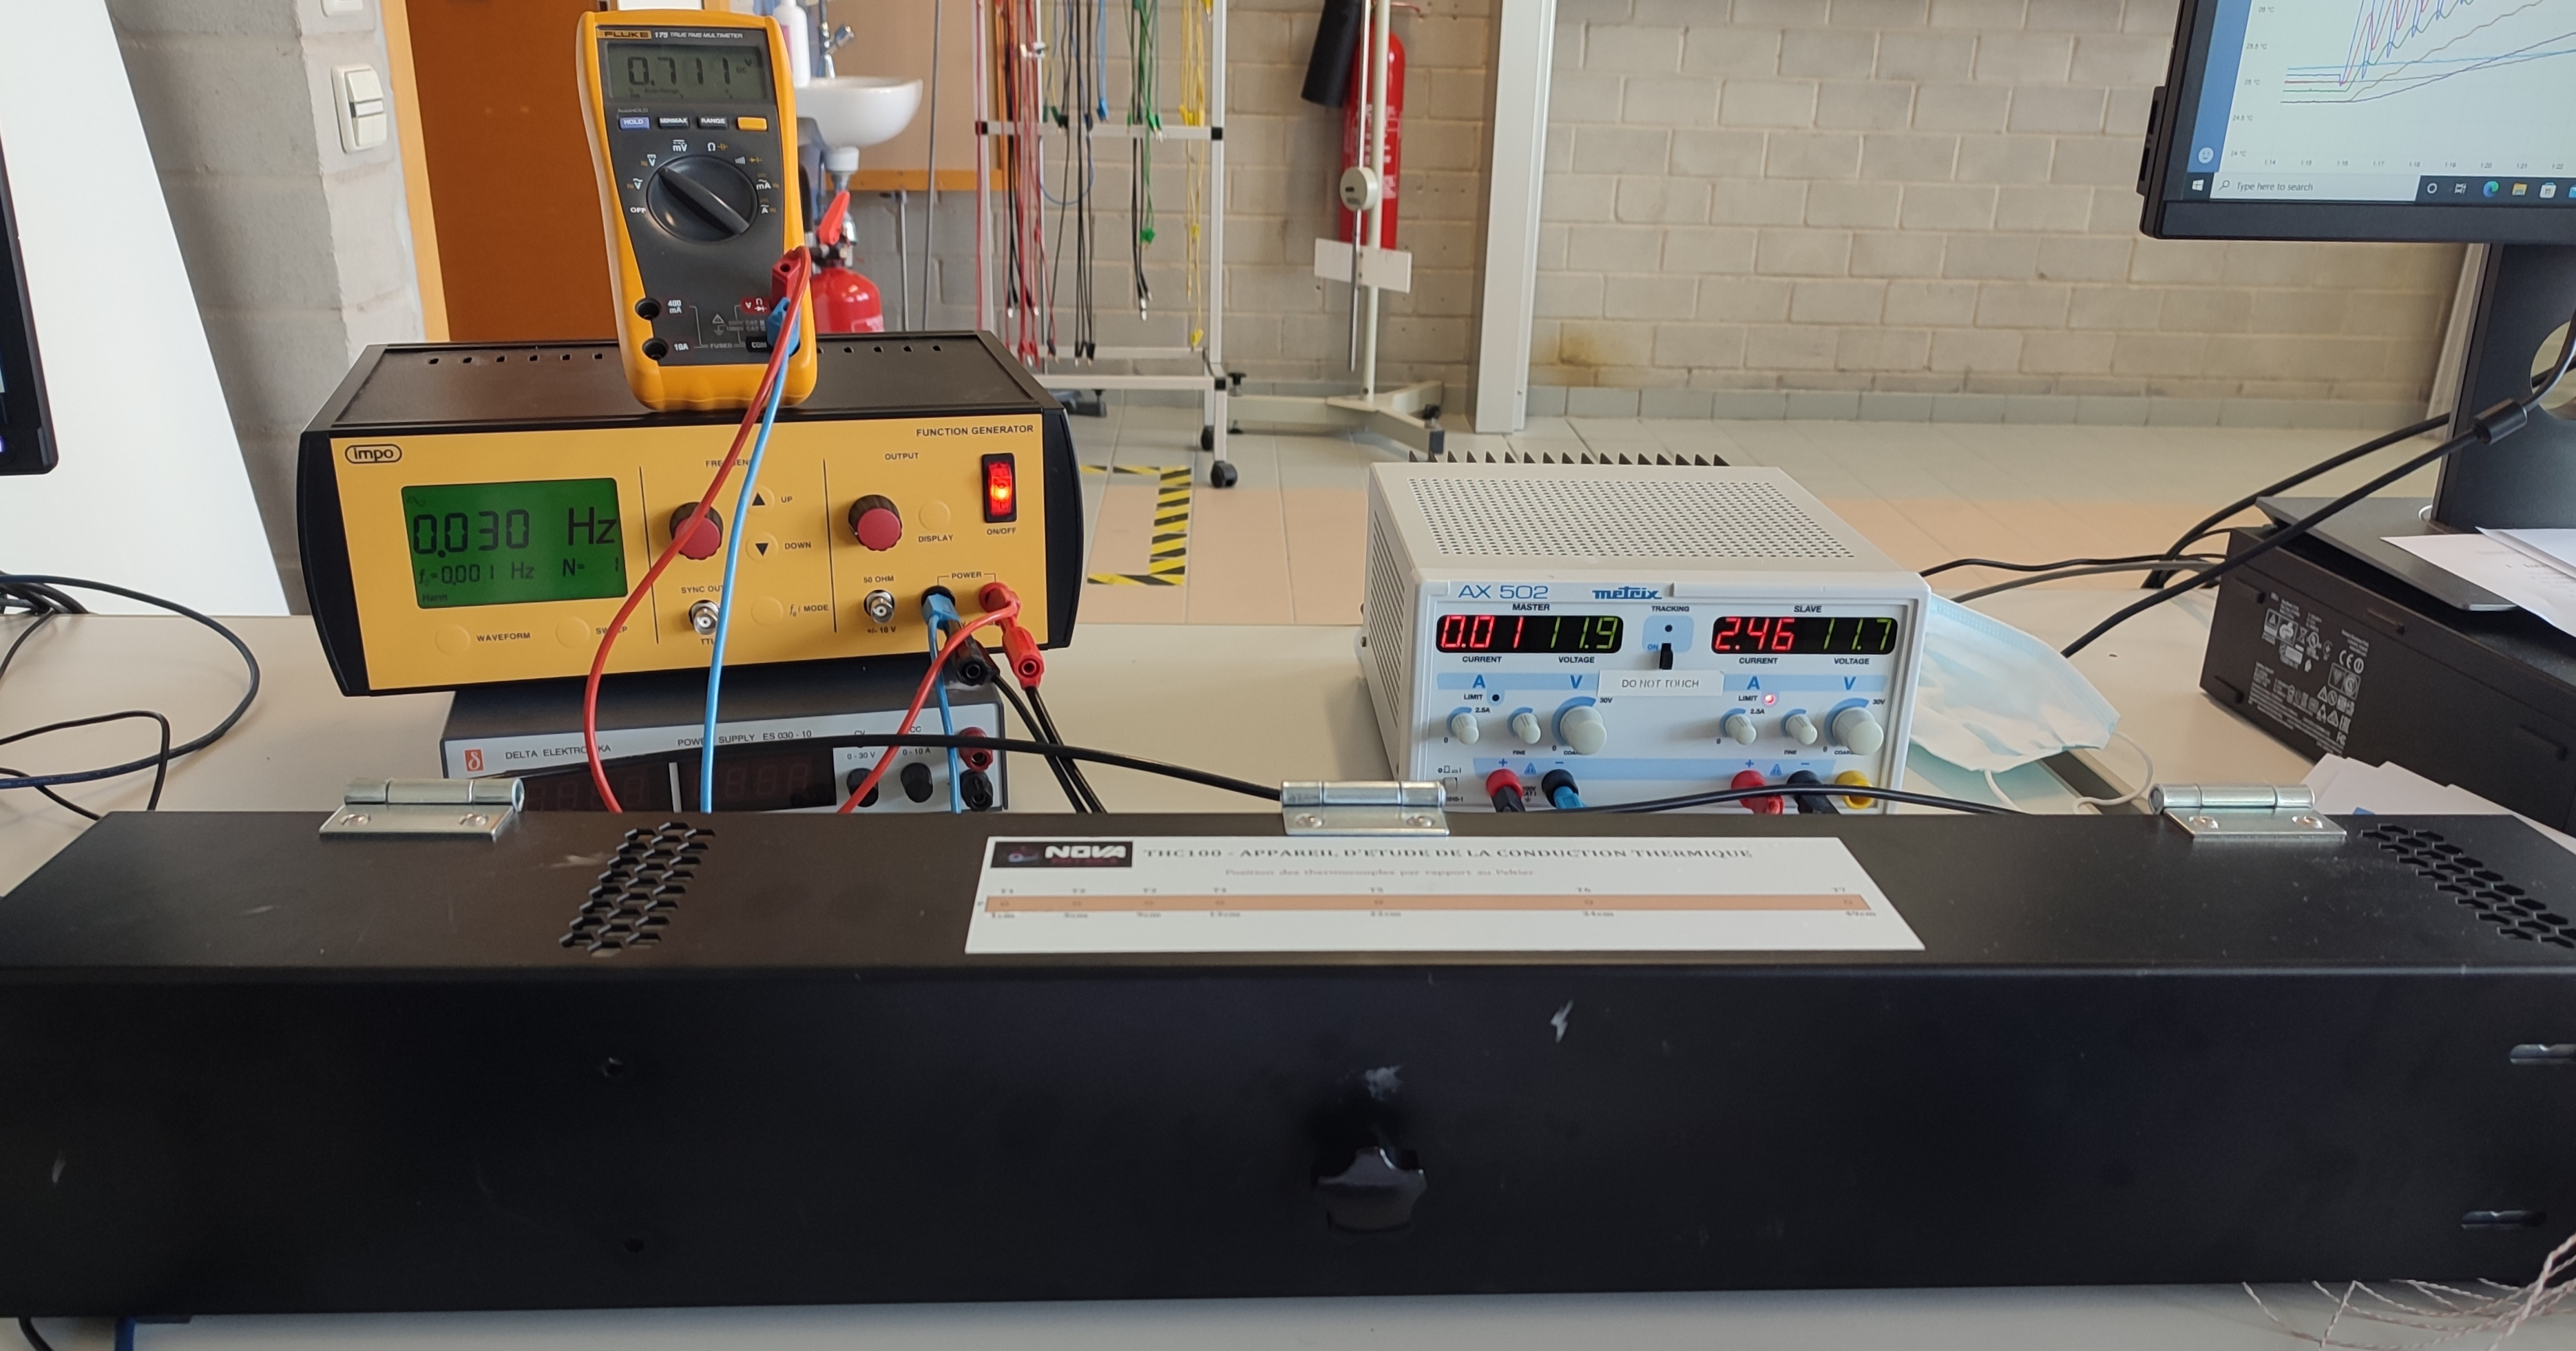
\includegraphics[width=0.7\textwidth]{Bilder/1652865310453.jpg}
    \caption{Experimental setup}
    \label{fig:setup}
\end{figure}

\subsection{Procedure}
\subsubsection{part I}
 For each temperature measurement, the amplitudes of the final oscillations, before the function generator was disconnected, are determined on the graph, using the relation:
\[A=\frac{T_{max}-T_{min}}{2}\]
We then take the average over the 4 measured values for the amplitude A for each temperature measurement and construct a graph displaying ln(A) as a function of the distance to the heat source of the thermalcouple, that took the measurement. When applying a linear fit, the slope is inversely proportional to the penetration depth $\delta$.
\[\delta = -\frac{1}{\text{slope}}\]
From there the thermal conductivity can be determined:
\begin{equation}
    \lambda = \delta^2\pi f\rho c_p
    \label{equation_lambda}
\end{equation}
where $\rho$ the density and $c_p$ the specific heat capacity of the sample.
This procedure is carried out for two different frequencies of the alternating current, 30 mHz and 3 mHz. 
\subsubsection{part II}
In the second part of the experiment the aim is to determine the thermal diffusivity as well as the thermal conductivity of aluminium by studying the transitional regime. 
First the final temperatures of each measurement position on the rod are noted. After a sufficient amount of time ($t\rightarrow\infty$), the solution of the heat equation:
\begin{equation}
    T(x,t)=T_1+(T_7-T_1)\frac{x}{L}-T_7a_0(x)e^{\frac{-t}{\tau}}
\end{equation}
reduces to:
\begin{equation*}
    T(x,\infty)=T_1+(T_7-T_1)\frac{x}{L}=T_{final}(x)
\end{equation*}
where $T_1$ is the temperature at the far left, i.e heated, end of the rod and $T_7$ the one on the far right and $\tau$ is the relaxation time, a measure of the time it takes for an object to be significantly perturbed, for which the following equation holds:
\begin{equation}
    \tau = \alpha_0^2\kappa^{-1}L^2
    \label{equ4}
\end{equation}
In order to determine $\tau$, we take linear fit of the plot of $\ln({T_{final}(x)-T(x,t)})$. The slope gives us $-\frac{1}{\tau}$.\\

Next we study the final temperature in the stationary state as a function of position. The graph is plotted and a linear fit is applied, where the slope gives us $\frac{\partial T}{\partial x}$. The relation:
\begin{equation}
  -\lambda \frac{\partial T}{\partial x}=-h(T_7-T_1)\quad\quad\Longleftrightarrow\quad\quad\frac{\lambda}{h}=\frac{T_7-T_1}{\frac{\partial T}{\partial x}}
\end{equation}
allows us to determine a value for the ratio $\frac{\lambda}{h}$, where h is an unknown constant. This step allows us to determine the constant $\alpha_0$ from equation \ref{equ4}, for which it can be shown that the following relation holds:
\begin{equation}
    \alpha_0\tan\alpha_0=L\frac{h}{\lambda}
    \label{equalpha}
\end{equation}
Using Desmos graphical calculator we plot the two functions $f_1(x)=x\tan x$ and $f_2(x)=L\frac{h}{\lambda}$ and find the value of x for which the functions intersect. The  x-coordinate of the first intersection point in the first quadrant gives us the value for $\alpha_0$.\\
Finally, using equation \ref{equ4} we can determine $\kappa$, and thereby $\lambda$:
\begin{equation}
    \lambda = \kappa\cdot\rho\cdot c_p
    \label{kappa}
\end{equation}
\section{Results}
\subsection{Harmonic regime}
\subsubsection{30 mHz}

The parameters applied on the generator are the following: \\
\textbf{frequency = 30 Hz and amplitude = 0.7 V}

With the recorded data we get the following plot:
\begin{figure}[H]
    \centering
    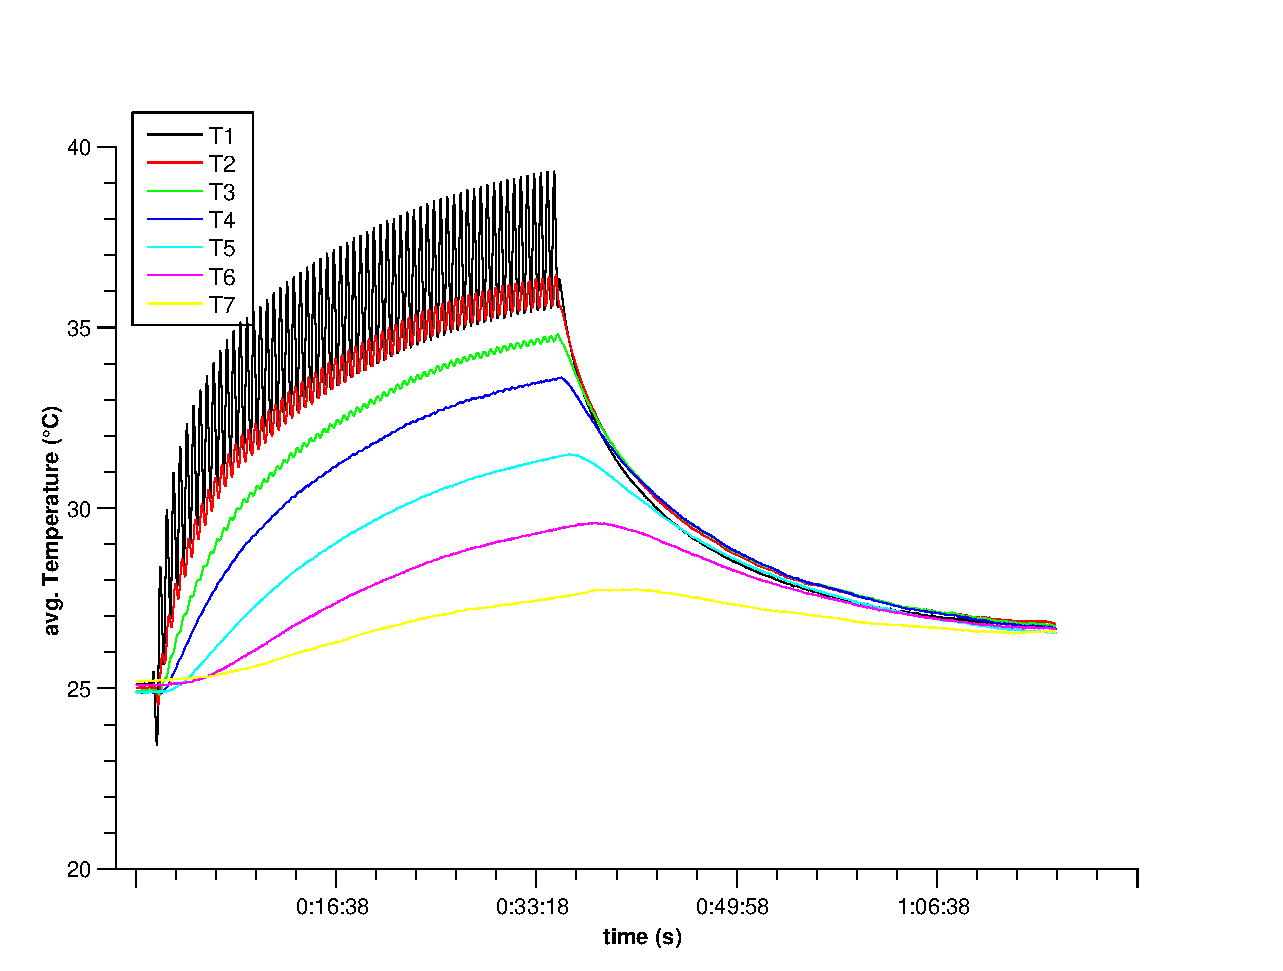
\includegraphics[width=0.7\textwidth]{30mHz.eps}
    \caption{Average temperature at different positions as a function of time for 30 mHz}
    \label{fig:30mHz}
\end{figure}
j

It was only possible to determine the amplitude for the three highest temperatures, since the others hadn't had a significant oscillatory motion.
\begin{table}[H]
    \centering
    \begin{tabular}{c|c|c}
        Temperature & Distance (cm) & Average amplitude A (°C) \\
        \hline
        T1 & 1 & 1.8762 \\
        T2 & 5 & 0.3925 \\
        T3 & 9 & 0.07 
    \end{tabular}
    \caption{Average amplitude for each temperature with respect to the distance for 30 mHz}
    \label{tab:30Hz_A}
\end{table}

Now plotting $\ln{A}$ as a function of the distance: 
\begin{figure}[H]
    \centering
    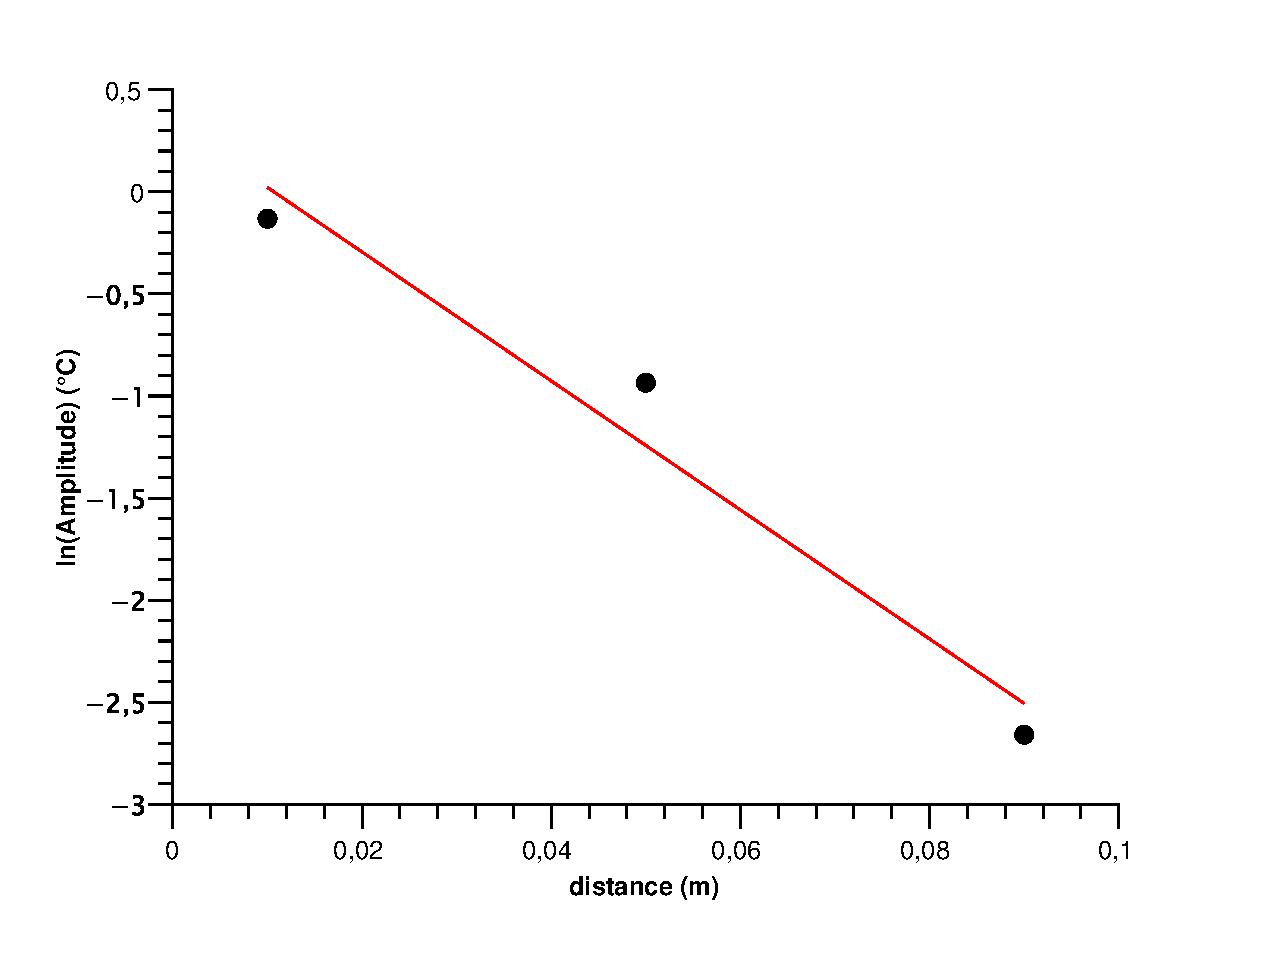
\includegraphics[width=0.6\textwidth]{ln_30mHz.eps}
    \caption{ln(A) as a function of the distance for 30 mHz}
    \label{fig:ln_30}
\end{figure}

The resulting slope corresponds to $s = (-31.588 \pm 6.65) \ m^{-1} $

Now $\delta = \frac{-1}{s} = 0.031657$ m. 
Having this result and knowing the frequency $f = 30 \ mHz$, the density of aluminium $\rho = 2.70 \cdot 10^3 \ \frac{kg}{m^3}$ and the the specific heat capacity $c_p = 900 \ \frac{J}{kg °C}$, we can calculate the heat conductivity using equation \ref{equation_lambda}.

\begin{align*}
    \lambda_{30 mHz} = 226.9763 \ \frac{W}{^{\circ}Cm}
\end{align*}

The theoretical thermal conductivity of aluminium is 237 W/m°C \cite{Theo_werte}. Which means our experimental results has a relative error of 4.2 \%.

\subsubsection{3 mHz}

The procedure is the same, only here we apply a frequency of 3 mHz and the amplitude stays the same.
The final plot is:

\begin{figure}[H]
    \centering
    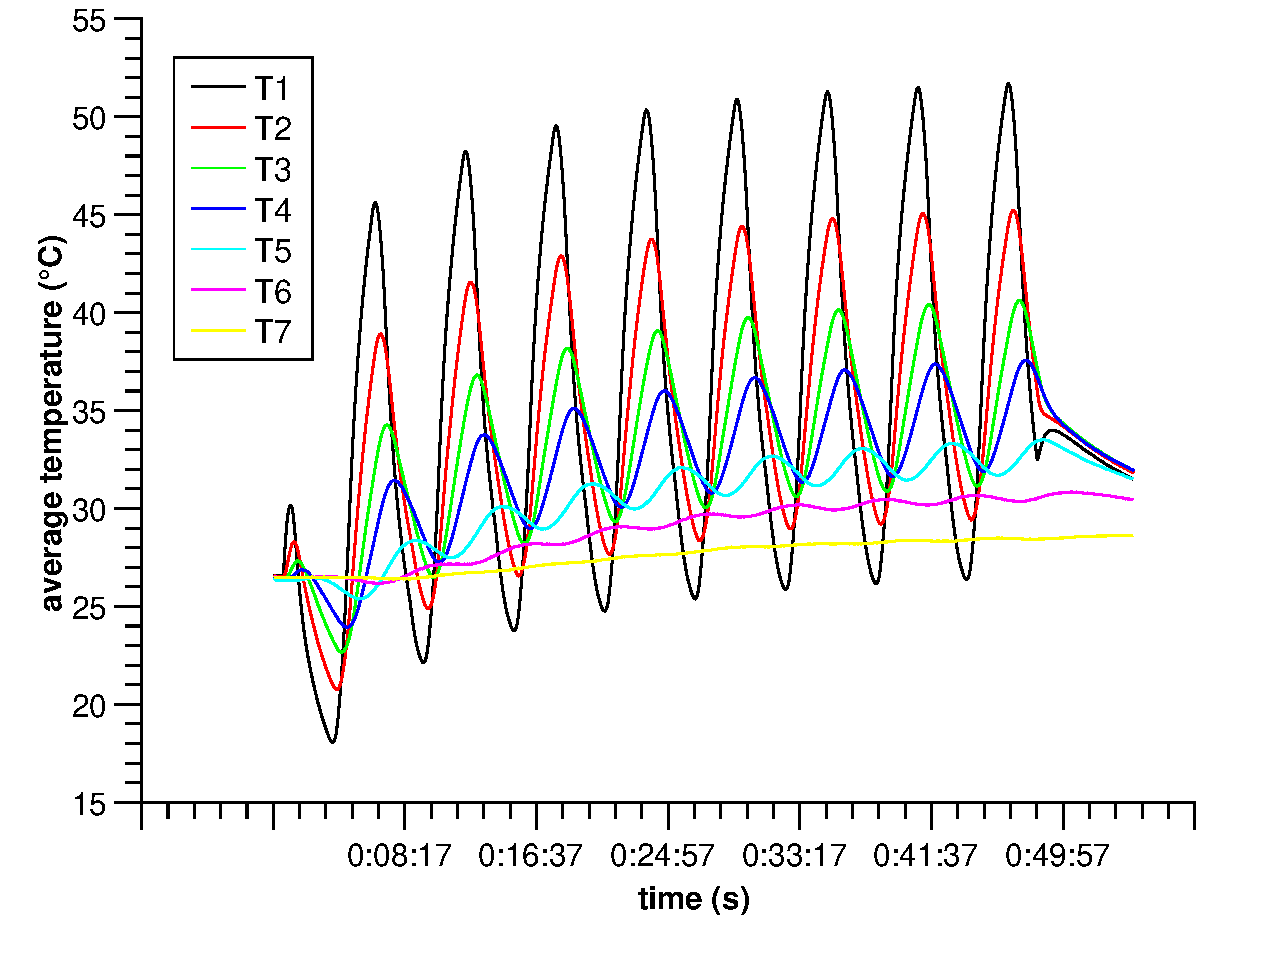
\includegraphics[width=0.7\textwidth]{3mHz.eps}
    \caption{Average temperature at different positions as a function of time for 3 mHz}
    \label{fig:3mHz}
\end{figure}

We determined the average amplitude for T1 up to T5, since the oscillations are clearly visible.
\begin{table}[H]
    \centering
    \begin{tabular}{c|c|c}
        Temperature & Distance (cm) & Average amplitude A (°C) \\
        \hline
        T1 & 1 & 12.42 \\
        T2 & 5 & 7.70 \\
        T3 & 9 & 4.58 \\
        T4 & 13 & 2.68 \\
        T5 & 22 & 0.77
    \end{tabular}
    \caption{Average amplitude for each temperature with respect to the distance for 3 mHz}
    \label{tab:30Hz_A}
\end{table}

Now plotting ln(A) against the distance:
\begin{figure}[H]
    \centering
    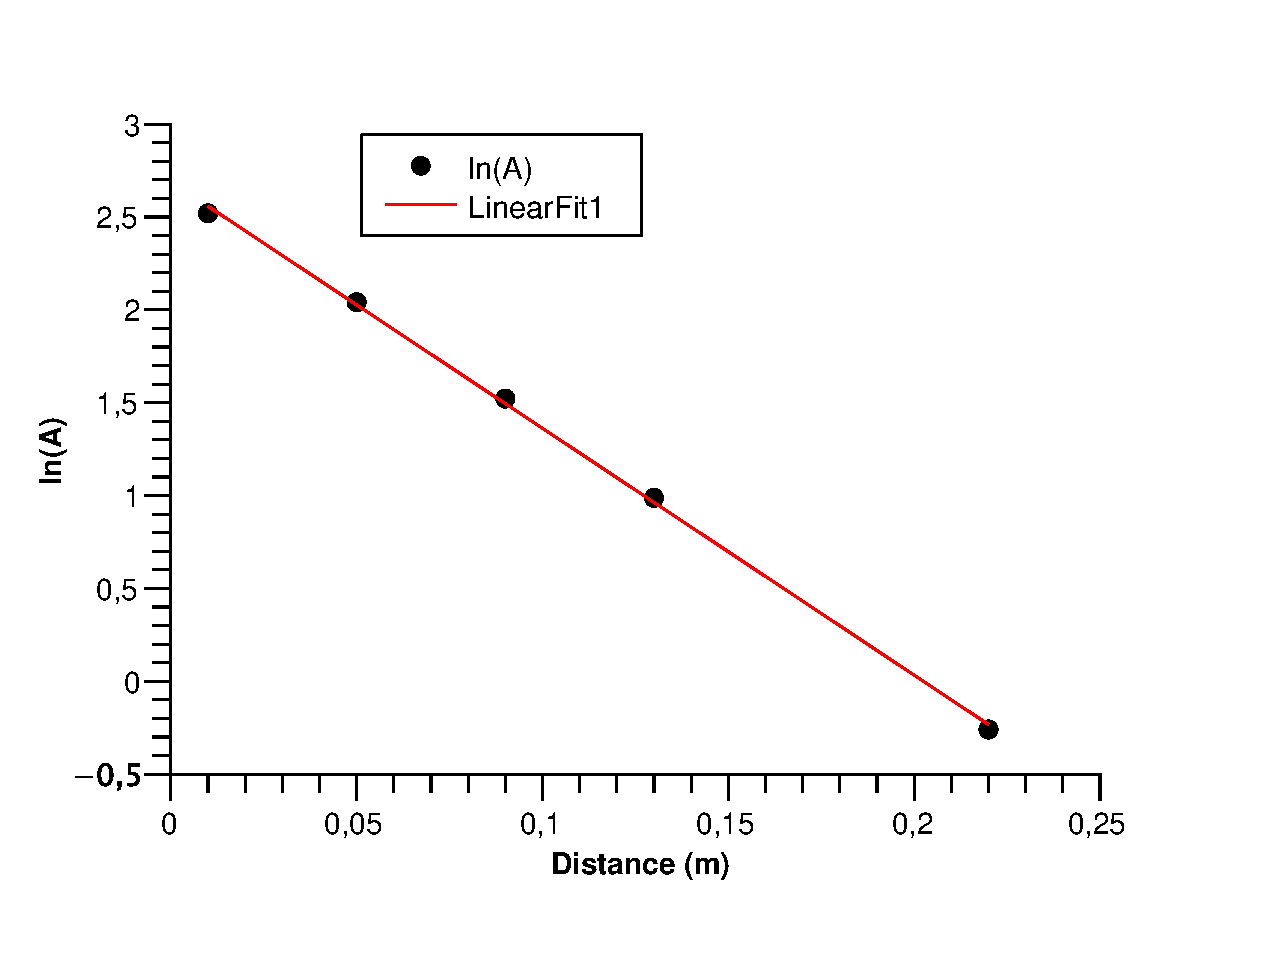
\includegraphics[width=0.7\textwidth]{ln_3mHz.eps}
    \caption{ln(A) as a function of the distance for 3 mHz}
    \label{fig:ln_3}
\end{figure}

The resulting slope is $s = (-13.29 \pm 0.21)  \ m^{-1}$, which gives us $\delta = \frac{-1}{s} = 0.07523$ m.\\

The thermal conductivity is:
\begin{equation*}
    \lambda_{3 mHz} = 129.61 \  \frac{W}{^{\circ}Cm}
\end{equation*}

This experimental result deviates from the theoretical one by 45.3 \%.
\newpage
\subsection{Transitional regime}
Plotting the average temperature recorded by the individual thermocouples:

\begin{figure}[!h]
    \centering
    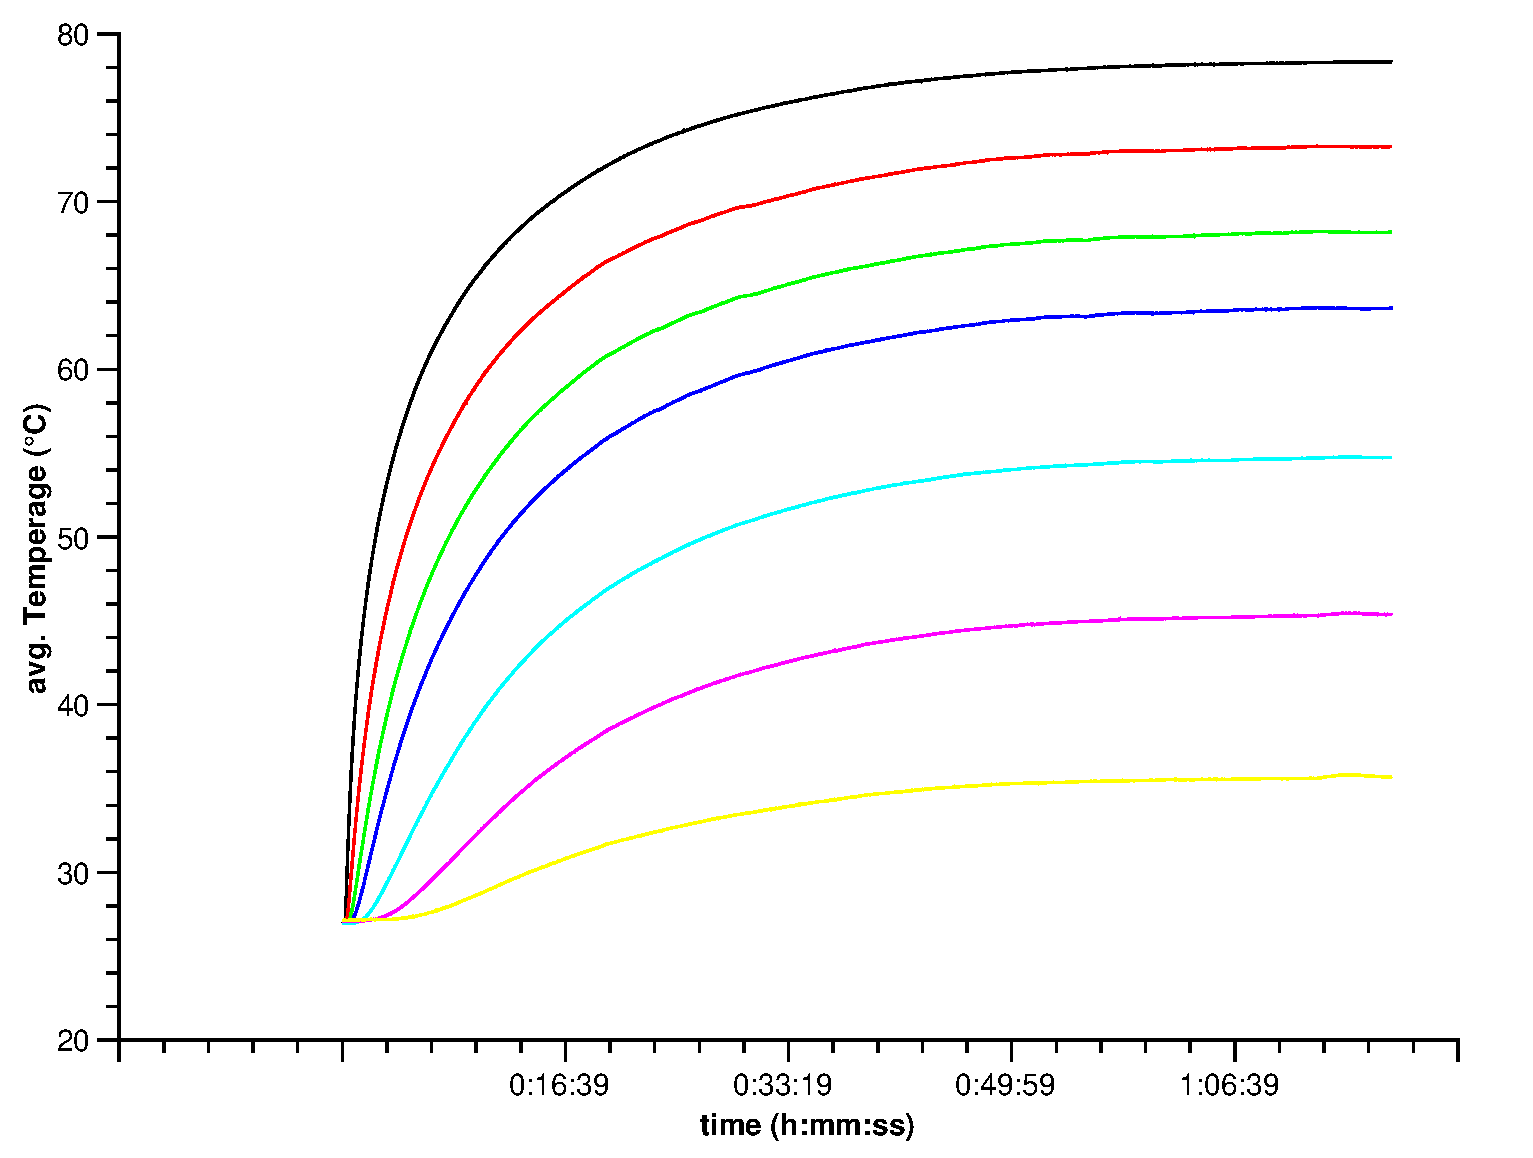
\includegraphics[width=0.7\textwidth]{avgT.eps}
    \caption{Avg. Temperatures}
    \label{fig:my_label}
\end{figure}

Reading off the final temperatures, the $\ln(T_f(x)-T(x,t))$ graph can be plotted. Taking the linear fit of the individual plots, the relaxation time $\tau$ can be obtained:

\begin{table}[H]%
\centering
\parbox{0.4\textwidth}{
\begin{footnotesize}
    \begin{tabular}{c|c|c}
        Measurement & $T_{final}$ ($^\circ$C) & $\tau$ (s)\\
        \hline
        $T_1$ & 78.33 & 822.57\\
        $T_2$ & 73.27 & 851.57\\
        $T_3$ & 68.18 & 850.85\\
        $T_4$ & 63.64 & 836.47\\
        $T_5$ & 54.75 & 830.70\\
        $T_6$ & 45.38 & 865.20\\
        $T_7$ & 35.70 & 915.51
    \end{tabular}
\end{footnotesize}
\caption{Relaxation time $\tau$}
\label{tab:table}
}
\qquad
\begin{minipage}[c]{0.53\textwidth}%
\centering
    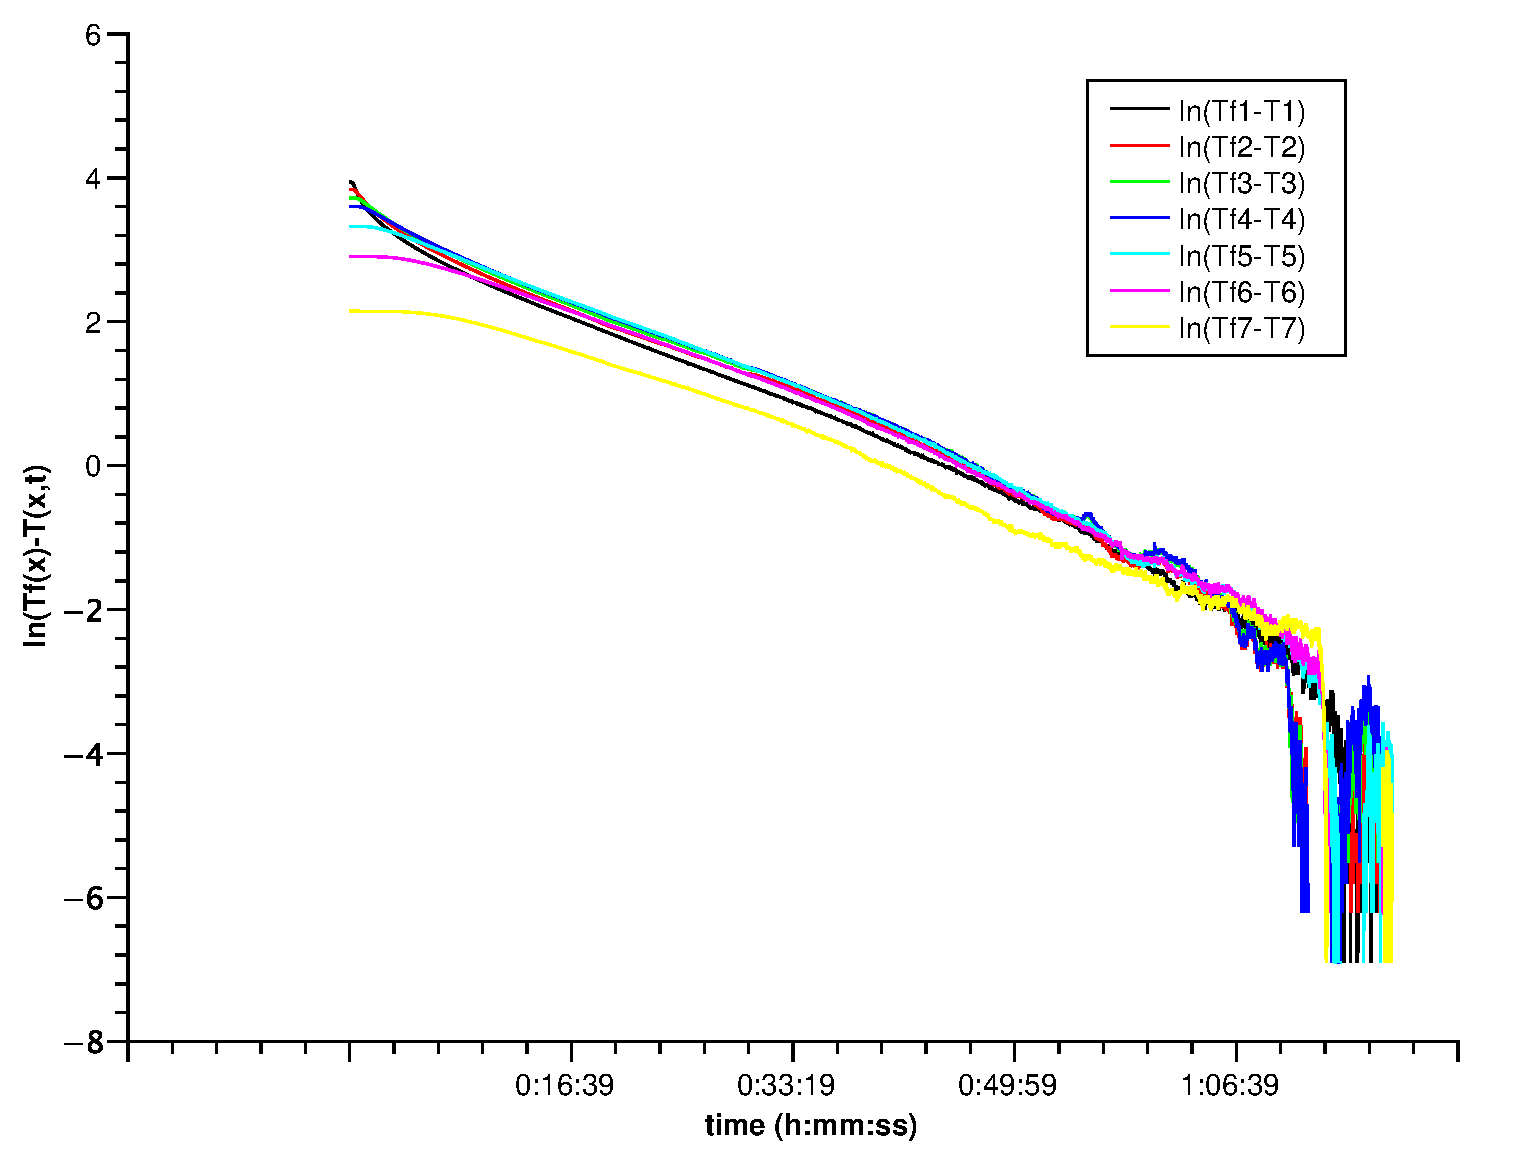
\includegraphics[width=1\textwidth]{lnTf_T.eps}
\caption{$\ln(T_f(x)-T(x,t))$}
\label{fig:figure}
\end{minipage}
\end{table}

Averaging over the individual values for $\tau$, the following value was obtained:
\[\tau=853.27 \ s\]

Plotting the final temperatures as a function of the position they were measured at and taking the linear fit:

\begin{figure}[H]
    \centering
    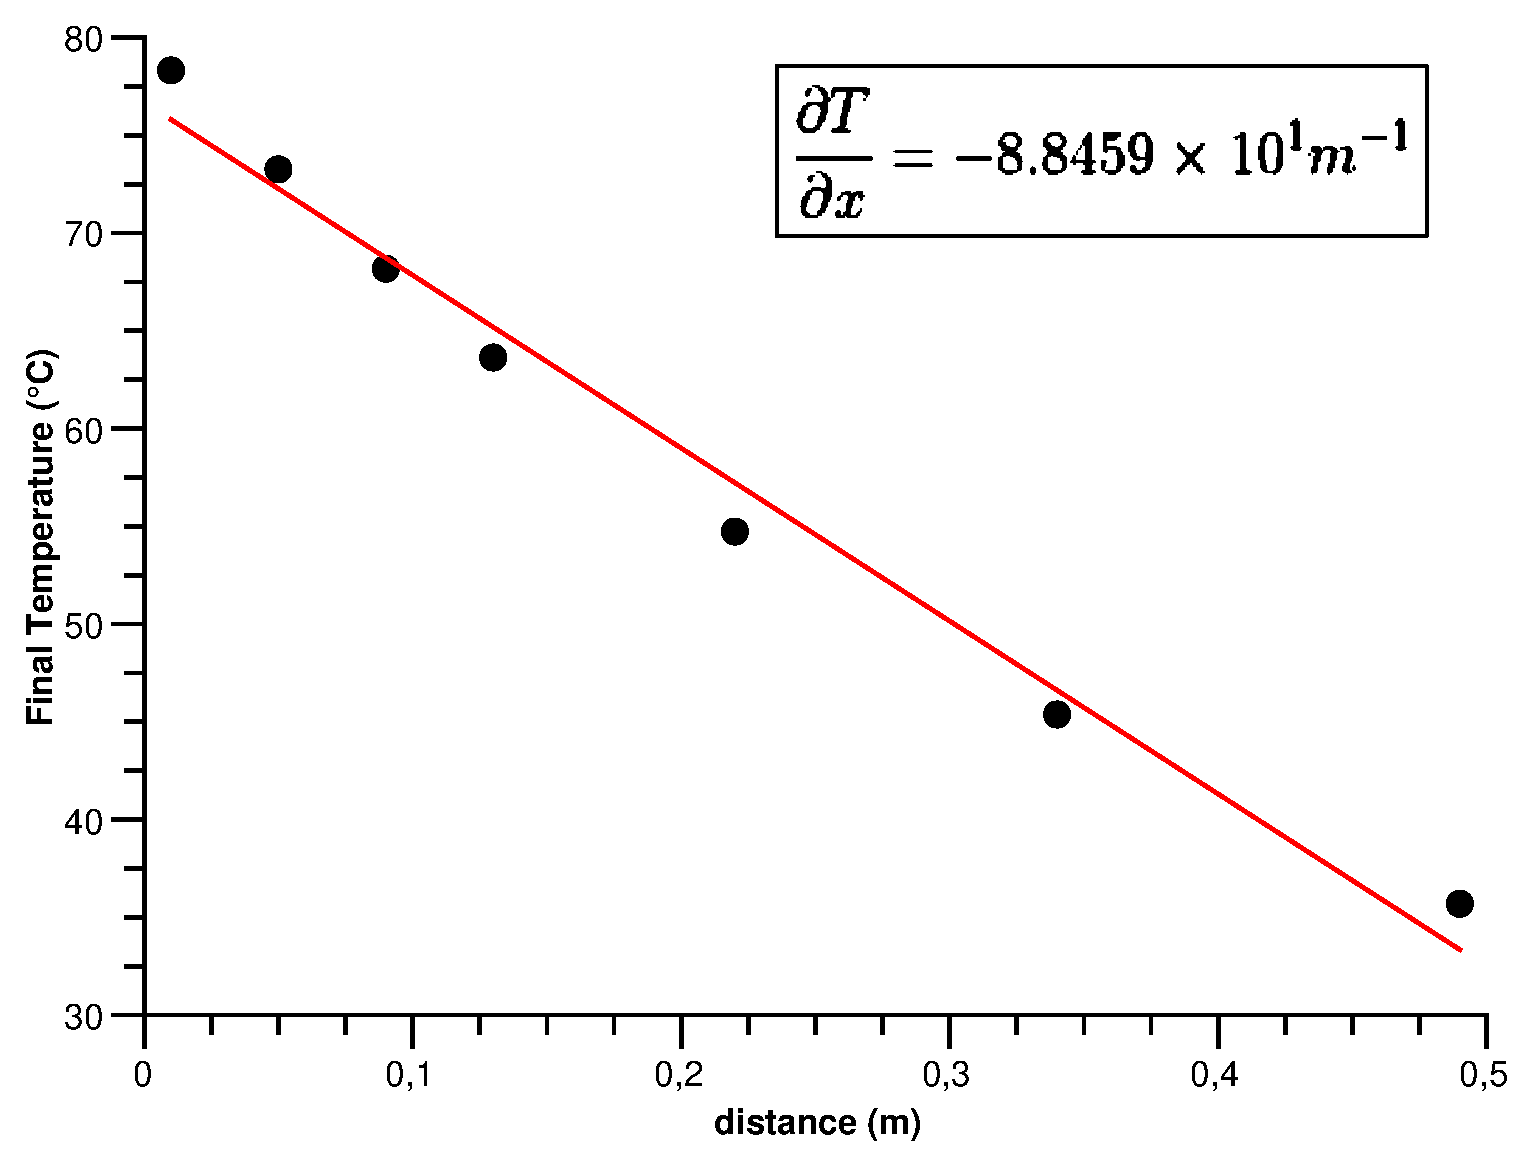
\includegraphics[width=0.7\textwidth]{gradientT.eps}
    \caption{Temperature Gradient}
    \label{fig:my_label}
\end{figure}

Hence, we determine:
\begin{align*}
    \frac{\lambda}{h} &=\frac{T_7-T_1}{\frac{\partial T}{\partial x}} =\frac{35.70^{\circ}C-78.33^{\circ}C}{-8.8459\cdot 10^1 m^{-1}} \\
    &=0.4819 \ m 
\end{align*}


\begin{wrapfigure}{r}{8cm}
    \centering
    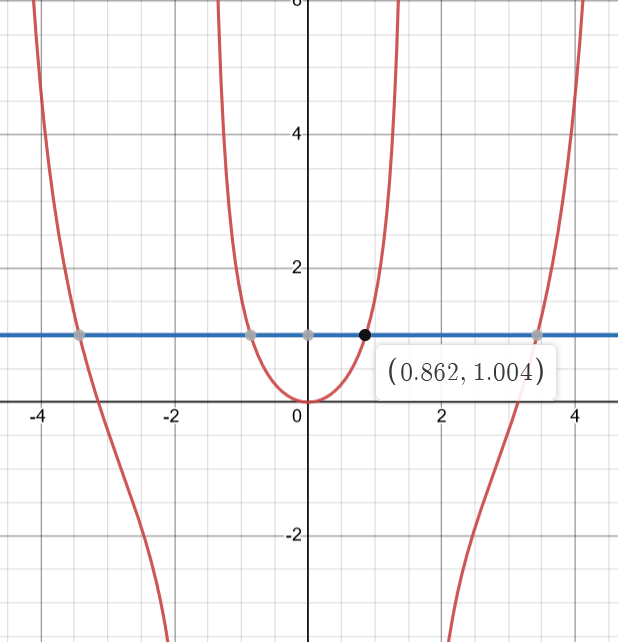
\includegraphics[width=0.4\textwidth]{xtanx.PNG}
    \caption{Graphical determination of $\alpha_0$}
    \label{fig:aplha0}
\end{wrapfigure}

We can now solve \ref{equalpha} graphically, with L=0.48m. Using Desmos graphical calculator, we find:
\begin{align*}
    \alpha_0\tan\alpha_0&=L\cdot\frac{h}{\lambda}=1.0040\\
    \Rightarrow\quad\alpha_0&=0.862
\end{align*}

\vspace{2cm}

Finally, using equation \ref{kappa} we can solve for the thermal diffusivity $\kappa$:
\[\kappa=\frac{L^2}{\alpha_0^2\tau}=267.90\ mm^2s^{-1}\]
Comparing to the literature value for aluminium:
\[\delta\kappa=\frac{|267.90-97.00|}{97.00}\times100=176.19\%\]
The large relative error is most probably due to an error on the determination of the relaxation time. Although the precision of the individual measurements is quite high, the accuracy might not. Moreover, as a lot of different quantities had to be determined in order to get to this value, error propagation plays an important factor. Furthermore, the temperatures $T_f$ might not be the real final temperatures, but only the final reading of the temperature, when we ended the measurement. Running the experiment for a longer amount of time would therefore also lead to better results.\\
The large error also propagates to the determination of the heat conductivity $\lambda$:
\begin{align*}
    \lambda &=\kappa\cdot\rho\cdot c_p = 643.76\ \frac{W}{^{\circ}Cm}\\
    \delta\lambda &=\frac{|643.76-237.00|}{237.00}\times100= 171.63\%
\end{align*}


\section{Conclusion}
In this lab class, we were able to determine the thermal conductivity of aluminium using two different regimes: the harmonic and transitional regime. For the harmonic regime of 30 mHz we got a really promising result for the thermal conductivity, 226.9763 W/°Cm with a relative error of only 4.2 \%. On the other hand, using a frequency of 3 mHz, we got 129.61 W/°Cm, which corresponds to a deviation of 45.3 \%. Actually, a better result should come out using 3 mHz, since the oscillations were more visible and therefore had more data for the computation.\\
Afterwards, using the transitional regime, we had to face several problems for the computation. Our technique is right, nevertheless we get an immense error of 171.63 \% on the thermal diffusivity. The error lies most likely in the calculation of the relaxation time $\tau$.



\begin{thebibliography}{}
\bibitem{Handout} Handout from the supervisor: \textit{Thermal conductivity} (version 1.4)
\bibitem{Theo_werte} \textit{Metals, Metallic Elements and Alloys - Thermal Conductivities}, TheEngineeringToolbox, \url{https://www.engineeringtoolbox.com/thermal-conductivity-metals-d_858.html}(visited 18/05/22)
\bibitem{effects} \textit{Thermoelectric effect}, Wikipedia, \url{https://en.wikipedia.org/wiki/Thermoelectric_effect#Seebeck_effect}(visited 18/05/22)

\end{thebibliography}

\end{document}
